\documentclass[tikz, border=1pt]{standalone}
\pdfoutput=1 % if your are submitting a pdflatex (i.e. if you have
             % images in pdf, png or jpg format)

\usepackage{graphicx}

% Use the tikz package
\usepackage{tikz}
\usetikzlibrary{decorations}


\begin{document}

        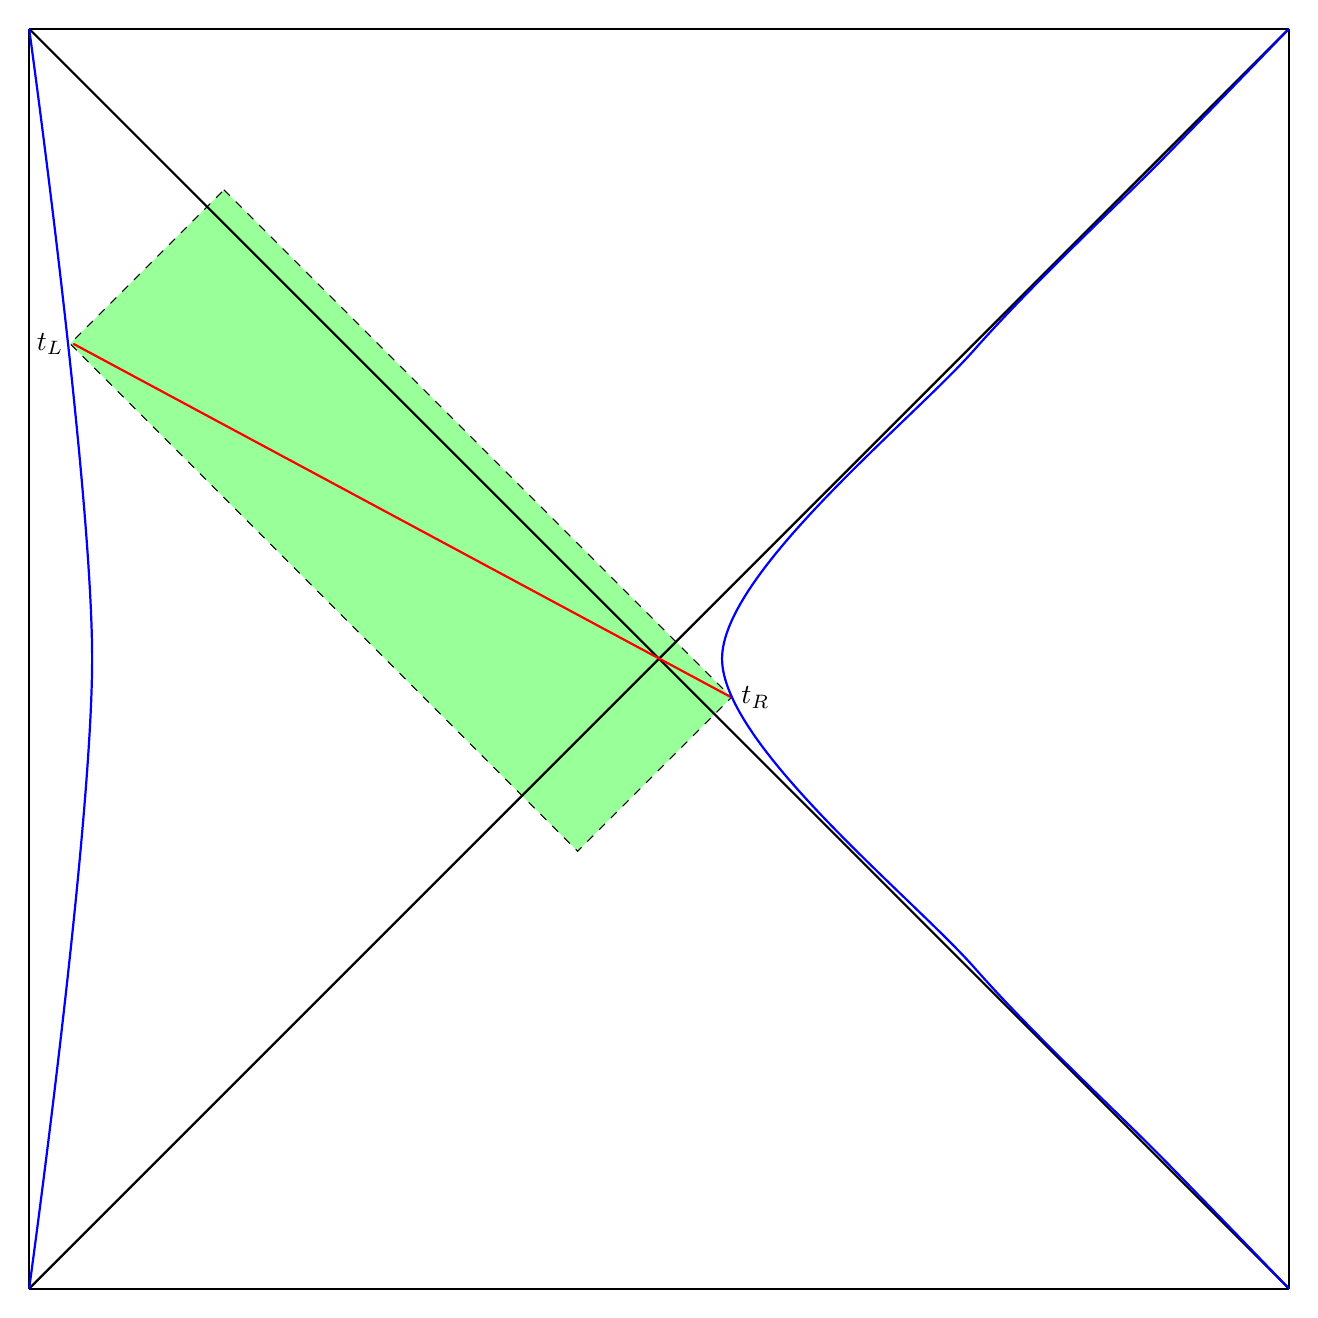
\begin{tikzpicture}[scale=4]
        
        % WdW boundaries
        \fill[green!40!white] (0.618503, 3.4885)--(2.23,1.87701)--(1.7415,1.3885)--(0.13,3)--(0.618503, 3.4885);
        \draw[dashed] (0.618503, 3.4885)--(2.23,1.87701)--(1.7415,1.3885)--(0.13,3)--(0.618503, 3.4885); 
        
        %axes
        \draw[thick] (0,0)--(4,0);
        \draw[thick] (4,0) --(4,4);
        \draw[thick] (4,4)--(0,4);
        \draw[thick] (0,4)--(0,0);
        \draw[thick] (0,0) --(4,4);
        \draw[thick] (0,4)--(4,0);
        
        \draw[thick][red] (0.14,3)--(2.23,1.87701);
        
        % cutoff
        \draw[blue,thick] plot [smooth] coordinates {(0,0) (0.2,2) (0,4)};
        \draw[blue,thick] plot [smooth] coordinates {(4,0) (3.6, 0.412549) (3,1.0202) (2.2,2) (3,2.9798) (3.6, 3.58745) (4,4)};
        
        %labels
        \draw (0.14,3) node[left]{$t_L$};
        \draw (2.23,1.87701) node[right]{$t_R$};
        
        \end{tikzpicture}

\end{document}
